\documentclass[tikz, crop, border = {2pt 2pt 2pt 2pt}]{standalone}

\usetikzlibrary{calc}
\usepackage{concmath-otf}

\begin{document}
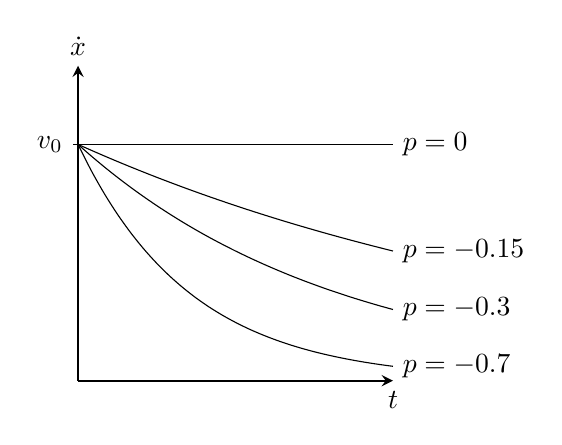
\begin{tikzpicture}
    \newcommand{\yscale}{3}
    \draw[-stealth, thick] (0, 0) -- (4, 0) node[below]{$t$};
    \draw[-stealth, thick] (0, 0) -- (0, 4) node[above]{$\dot{x}$};

    \foreach \x in {0, -0.15, -0.3, -0.7} {
        \draw[smooth, variable = \t, domain = 0:4] plot (\t, {\yscale*e^(\x*\t)}) node[right]{$p = \x$};
    }
    
    \draw (2pt, 3) -- ++ (-4pt, 0) node[left]{$v_0$};
\end{tikzpicture}
\end{document}